% @Author: AnthonyKenny98
% @Date:   2020-02-22 15:53:59
% @Last Modified by:   AnthonyKenny98
% @Last Modified time: 2020-04-05 18:38:15


% TECHNICAL SPECIFICATIONS
\subsection{Technical Specifications}

    With \gls{RRT} selected as the benchmark algorithm against which to test specialised hardware, this project required an implementation of the algorithm that satisfied the following criteria shown in Table \ref{table:RRT_Tech_Specs_Abbrev}. Appendix \ref{section:rrt_appendix_tech_specs} is a more thorough description of the technical specifications for the implementation of RRT. 

    % Tech Spec Table
    \begin{table}[H]
\begin{center}
\begin{tabular}{|p{.3\linewidth}|p{.64\linewidth}|}
    \hline
    Requirement             & Description and Justification \\
    \hline
    C/C++ Implementation    & As outlined in Section \ref{subsection:project_structure}, the critical step in determining the design of specialized hardware to accelerate \ac{RRT} is CPU performance analysis of the algorithm to determine computational hot-spots. Implementations in C allow for the use of certain CPU profiling tools, described in Section \ref{subsubsection:vtune}, unlike higher-level languages such as Python. \\
    \hline
    Models Drone as Point   & In reality, implementing \ac{RRT} for a drone would model the robot as a \ac{3D} object defined by coordinates $\{x, y, z\}$ and Euler angles $\{\alpha, \beta, \gamma \}$. However, for simplicity's sake, modelling the drone as a point defined by coordinates $\{x, y, z\}$ will suffice. Time permitting, this could be revisited. \todo[inline]{Change this based on whether time does permit} \\
    \hline
    Mirrors Algorithm       & In order for the results of CPU performance analysis to be easy to understand, software implementation of \ac{RRT} should call functions that mirror the functions described in Algorithms \ref{algorithm:rrt} and \ref{algorithm:rrt_collision}. \\
    \hline
\end{tabular}
\caption{Technical Specifications for \ac{RRT} Implementation}
\label{table:RRT_Tech_Specs}
\end{center}
\end{table}
\todo[inline]{Improve this table}

    The original intention was to find an existing implementation of RRT that could fulfill these requirements. However, no open-source implementations were suitable. Appendix \ref{section:rrt_appendix_existing_implementations} shows an evaluation of existing implementations.

    As a result, it was necessary to build a C implementation of RRT from the ground up to the aformentioned specifications.

\subsection{Implementation Design}
    
    The design and implementation of \gls{RRT}, while neccessary, was significant and time consuming. Since this was not the main object of this thesis, only a brief description of key design choices has been included here. Appendix \ref{appendix:rrt_appendix} contains a more detailed account.

    \subsubsection{Parameterization}
        Table \ref{table:rrt_params} shows the parameters that were included in the implementation and compiled by way of a C header file.
        % @Author: AnthonyKenny98
% @Date:   2020-04-05 17:54:44
% @Last Modified by:   AnthonyKenny98
% @Last Modified time: 2020-04-11 01:49:58
\begin{table}[H]
\begin{centering}
\begin{tabular}{|c|c|l|}
\hline
\textbf{Parameter} & \textbf{Data Type} & \textbf{Description} \\
\hline
$\epsilon$ & Integer & Maximum distance between two configurations \\
\hline
$K$ & Integer & Maximum number of configurations in the graph \\
\hline
$DIM$ & Integer & Upper bound of each axis of workspace \\
\hline
Goal Bias & Float & Percentage likelihood of stepping towards goal node \\
\hline
\gls{OGM} & File Pointer & \glsname{CSV} of booleans to represent grids \\
\hline
\end{tabular}
\mycaption{RRT Implementation Parameters}{}
\label{table:rrt_params}

\end{centering}
\end{table}

    \subsubsection{Key Functions}
        Algorithm \ref{algorithm:rrt_collision} shows that there are 5 key functions that constitute \gls{RRT}. Figure \ref{fig:rrt_functions} demonstrates each of these functions: \texttt{getRandomConfig()}, \texttt{findNearestConfig()}, \texttt{stepFromNearest()}, \texttt{(configCollisions)}, and \texttt{edgeCollisions()}.
        % @Author: AnthonyKenny98
% @Date:   2020-04-05 18:33:38
% @Last Modified by:   AnthonyKenny98
% @Last Modified time: 2020-04-05 19:45:01
\begin{figure}[t!]
\begin{centering}
\begin{tabular}{ccc}

    \begin{subfigure}{0.3\linewidth}
    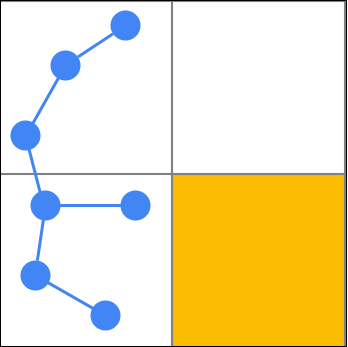
\includegraphics[width=\linewidth]{chapters/chapter2/img/keyfunctions/functions1.png}
    \caption{\texttt{getRandomConfig()}}
    \label{rrt_functions_a}
    \end{subfigure} & 

    \begin{subfigure}{0.3\linewidth}
    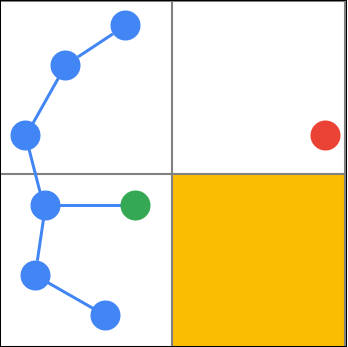
\includegraphics[width=\linewidth]{chapters/chapter2/img/keyfunctions/functions2.png}
    \caption{\texttt{findNearestConfig()}}
    \label{rrt_functions_b}
    \end{subfigure} &

    \begin{subfigure}{0.3\linewidth}
    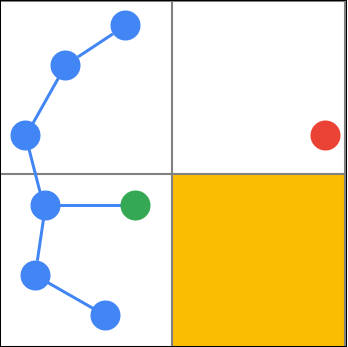
\includegraphics[width=\linewidth]{chapters/chapter2/img/keyfunctions/functions3.png}
    \caption{\texttt{stepFromNearest()}}
    \label{rrt_functions_c}
    \end{subfigure} \\

    \begin{subfigure}{0.3\linewidth}
    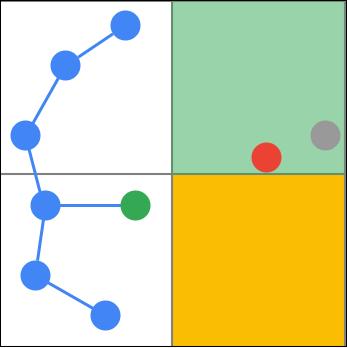
\includegraphics[width=\linewidth]{chapters/chapter2/img/keyfunctions/functions4.png}
    \caption{\texttt{configCollision()}}
    \label{rrt_functions_d}
    \end{subfigure} &

    \begin{subfigure}{0.3\linewidth}
    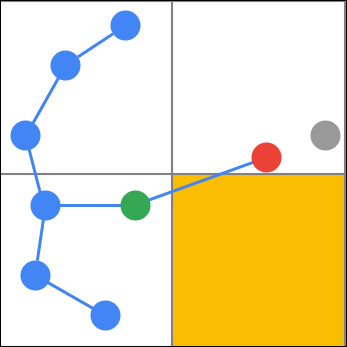
\includegraphics[width=\linewidth]{chapters/chapter2/img/keyfunctions/functions5.png}
    \caption{\texttt{edgeCollision()}}
    \label{rrt_functions_e}
    \end{subfigure} & 

    \begin{subfigure}{0.3\linewidth}
    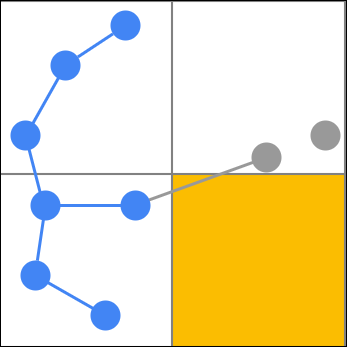
\includegraphics[width=\linewidth]{chapters/chapter2/img/keyfunctions/functions6.png}
    \caption{Discard}
    \label{rrt_functions_f}
    \end{subfigure} \\

\end{tabular}
\caption[Demonstration of the 5 Key Functions that Constitute RRT]{\textbf{Demonstration of the 5 Key Functions that Constitute RRT}, where configuration is a node in a 2D workspace. A new node is generated in (a) with \texttt{getRandomConfig()}, and the closest existing node is found with \texttt{findNearestConfig()} in (b). In this case, the new node is further that $\epsilon$ from the nearest node, and so a new node is generated with \texttt{stepFromNearest()} in (c). \texttt{configCollision} determines that the new node is not in an occupied grid (d) and draws an edge between the two nodes. \texttt{edgeCollision()} determines that, in this case, there is a collision (e) and the new node is discarded (f).}
\label{fig:rrt_functions}
\end{centering}
\end{figure}

    \subsubsection{Dimensionality}

    \subsubsection{$K$:DIM Ratio}

\subsection{Visualizing Implementation}
% @Author: AnthonyKenny98
% @Date:   2020-02-23 14:14:12
% @Last Modified by:   AnthonyKenny98
% @Last Modified time: 2020-03-01 08:06:12


\begin{figure}[H]
\begin{center}
\begin{tabular}{c  c}
    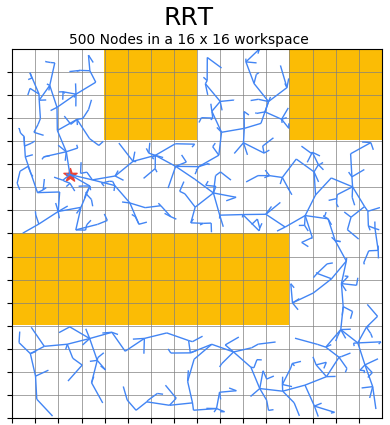
\includegraphics[width=0.45\linewidth]{chapters/chapter2/img/rrt_2d_1.png} & 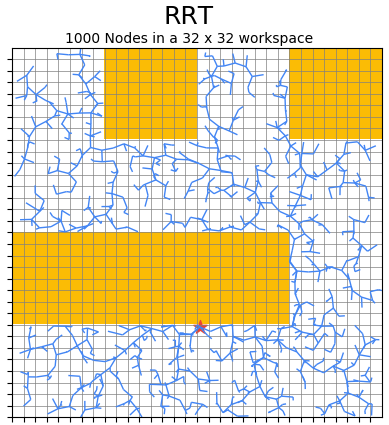
\includegraphics[width=0.45\linewidth]{chapters/chapter2/img/rrt_2d_2.png} \\
    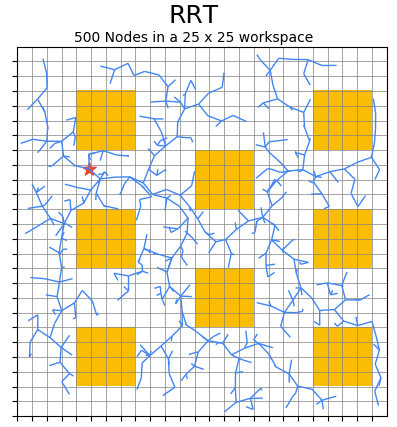
\includegraphics[width=0.45\linewidth]{chapters/chapter2/img/rrt_2d_3.png} & 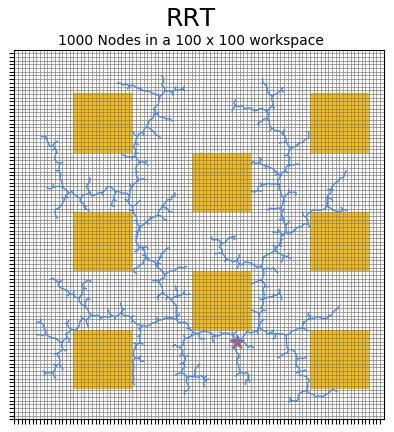
\includegraphics[width=0.45\linewidth]{chapters/chapter2/img/rrt_2d_4.png}
    \end{tabular}
    \caption{2D RRT Implementation shown by \ac{GUI}}
    \label{figure:2DrrtGui}
\end{center}
\end{figure}

\todo[inline]{Describe implementation in 3D}
% @Author: AnthonyKenny98
% @Date:   2020-02-23 14:14:12
% @Last Modified by:   AnthonyKenny98
% @Last Modified time: 2020-03-01 13:51:49


\begin{figure}[H]
\begin{center}
    \begin{tabular}{c  c}
    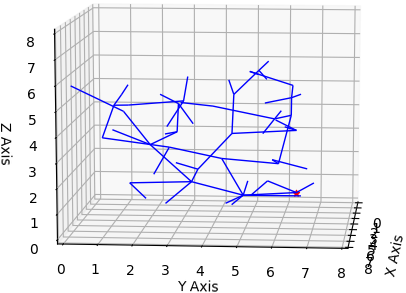
\includegraphics[width=0.45\linewidth]{chapters/chapter2/img/rrt_3d_1.png} & 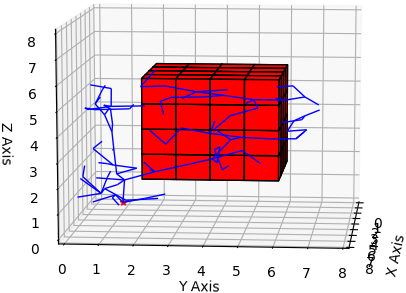
\includegraphics[width=0.45\linewidth]{chapters/chapter2/img/rrt_3d_2.png} \\
    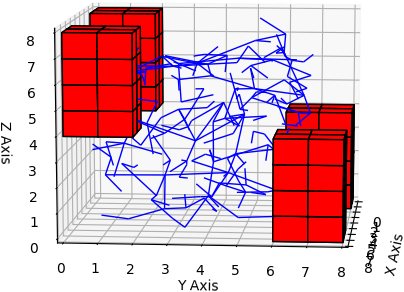
\includegraphics[width=0.45\linewidth]{chapters/chapter2/img/rrt_3d_3.png} & 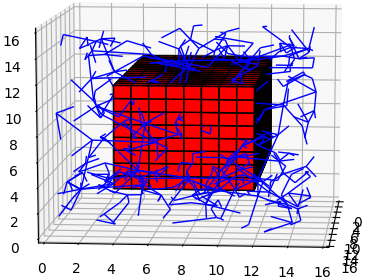
\includegraphics[width=0.45\linewidth]{chapters/chapter2/img/rrt_3d_4.png}
    \end{tabular}
    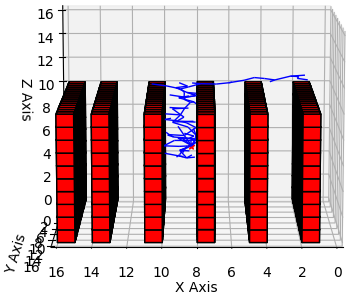
\includegraphics[width=0.45\linewidth]{chapters/chapter2/img/rrt_3d_5.png}
    \caption{3D RRT Implementation shown by \ac{GUI}}
    \label{figure:3DrrtGui}
\end{center}
\end{figure}
